\documentclass[a4paper]{article}
\usepackage[utf8]{inputenc}
\usepackage{graphicx}
\usepackage{epstopdf}
\usepackage{epsfig}
\usepackage{wrapfig}
\usepackage{subcaption}
\usepackage{float}
\usepackage{listings}
\usepackage[english,serbian]{babel}
\usepackage[usenames,dvipsnames]{color}

% This is the color used for MATLAB comments below
\definecolor{MyDarkGreen}{rgb}{0.0,0.4,0.0}

% For faster processing, load Matlab syntax for listings
\lstloadlanguages{Matlab}%
\lstset{language=Matlab,                        % Use MATLAB
        frame=single,                           % Single frame around code
        basicstyle=\small\ttfamily,             % Use small true type font
        keywordstyle=[1]\color{Blue}\bfseries,        % MATLAB functions bold and blue
        keywordstyle=[2]\color{Purple},         % MATLAB function arguments purple
        keywordstyle=[3]\color{Blue}\underbar,  % User functions underlined and blue
        identifierstyle=,                       % Nothing special about identifiers
                                                % Comments small dark green courier
        commentstyle=\usefont{T1}{pcr}{m}{sl}\color{MyDarkGreen}\small,
        stringstyle=\color{Purple},             % Strings are purple
        showstringspaces=false,                 % Don't put marks in string spaces
        tabsize=5,                              % 5 spaces per tab
        %
        %%% Put standard MATLAB functions not included in the default
        %%% language here
        morekeywords={xlim,ylim,var,alpha,factorial,poissrnd,normpdf,normcdf},
        %
        %%% Put MATLAB function parameters here
        morekeywords=[2]{on, off, interp},
        %
        %%% Put user defined functions here
        morekeywords=[3]{FindESS, homework_example},
        %
        morecomment=[l][\color{Blue}]{...},     % Line continuation (...) like blue comment
        numbers=left,                           % Line numbers on left
        firstnumber=1,                          % Line numbers start with line 1
        numberstyle=\tiny\color{Blue},          % Line numbers are blue
        stepnumber=5                            % Line numbers go in steps of 5
}

\begin{document}

\title{Logistička modifikacija Lotka-Voltera modela\\
	\small{Seminarski u okviru kursa\\Osnove matematičkog modeliranja\\Matematički fakultet}
}
\author{Marina Brkić, Nikola Vlahović\\marinabrkic91@gmail.com\\nikola.vlahovic2401@gmail.com}
\date{27. ~maj 2018.}
\maketitle
\abstract{
	Lotka-Voltera nelinearne diferencne jednačine prvog reda
	se koriste za modeliranje bioloških, hemijskih i ekonomskih sistema.
	Kroz primer interakcije lisica i zečeva, predstavljamo standardne jednačine i
	modifikaciju koja uzima u obzir ograničen kapacitet staništa.

	Ključne reči: Lotka-Voltera jendačine, modeliranje populacija, predator-plen
}
\tableofcontents

\newpage

\section{Uvod}
\label{sec:uvod}

Alfred J. Lotka je u svom radu "Doprinos teoriji periodičnih reakcija" objavljenom 1910. godine predstavio
inicijalnu formulaciju Lotka-Voltera jednačina za modeliranje ponašanja određenih hemijskih reakcija, koju
1920. koristi za modeliranje sistema u kom interaguju biljka i biljojed. Pet godina kasnije objavljuje knjgu
gde pomoću ovih jednačina modelira populacije plena i grabljivice. Te jednačina objavljuje i Vito Voltera
u radu gde analizira populacije riba u Jadranskom moru, nakon što je kroz razgovor sa svojim budućim zetom,
morskim biologom Umbertom D'Ankonom, saznao da je nakon rata porastao procenat ulovljenih grabljivih riba.
\\\\
Ilustrovaćemo kroz primer lisica i zečeva primenu Lotka-Voltera jednačina na modeliranje
populacija sa plen-grabljivica interakcijama.

\section{Standardni Lotka-Voltera model}
\label{sec:std_model}
Stanište dele populacije lisica i zečeva. Lisice se hrane isključivo zečevima,
dok za zečeve uvek ima hrane u izobilju. Populacija zečeva bi u nedostatku lisica
neprestano rasla. Obratno, populacija lisica bi u slučaju nedostatka zečeva (hrane) ubrzo izumrla.
Označimo broj zečeva sa x(t), a broj lisica sa y(t) za vreme t.
Jednačine:
	\begin{center}
	$x' = ax$ \\
	$y' = -my$
	\end{center}
gde su a i m parametri koji predstavljaju stope rasta i odumiranja odgovarajućih populacija,
ilustruju njihovo ponašanje u nedostatku interakcije.
Da bismo dobili realističniji model, neophodno je da inkorporiramo u jednačine
činjenicu da lisice love zečeve. Broj njihovih susreta je direktno proporcionalan
brojnosti lisica i zečeva, što možemo modelirati proizvodom xy. Lov izaziva opadanje
populacije zečeva, dok omogućava porast. Neka su b i c koeficijenti smrtnosti zečeva tj.
nataliteta lisica pri omogućenim interakcijama, i pretpostavimo da su lisice nezasite,
tj. da će svaku priliku iskoristiti da pojedu zeca.
Promene populacija možemo modelirati \textbf{Lotka-Voltera sistemom diferencnih jednačina}:
		\begin{center}
		$x' = ax - bxy,   x(0)=x_0$\\
		$y' = -my + cxy,  y(0)=y_0$
		\end{center}

Analitičko rešenje ovog sistema je teško naći i zbog toga se koriste numeričke metode.
Iz jednačina sledi da će porast populacije zečeva kao posledicu omogućiti porast populacije lisica,
ali kako populacija lisica raste tako dolazi i do povećannja konzumacije zečeva, usled koje će eventualno
početi da se smanjuje broj zečeva.
Kako se bude smanjivala količina hrane za lisice, tako će i njihov broj morati da opadne.
Postiže se \textbf{ravnotežno stanje} kada se brojnost ni jedne populacije ne menja (x'=0 i y'=0).
Postoji po jedno pozitivno ravnotežno stanje za obe jednačine, i to su $x=m/c$ iz jednačine za zečeve i $y=a/b$, iz jednačine za lisice.\\
Zaključujemo da  graf sa tačkama (x(t),y(t)) mora biti zatvorena kriva.
Da bi ovo videli, razmotrimo funkciju:
\begin{center}
	$H(x,y)=c ln(y) - my + a ln(x) - bx$
\end{center}
Diferenciramo i dobijamo:
\begin{center}
	$H'=H_y y' + H_x x' = (b/y - c)(-d + mx)y + (d/x - m)(b - cy)x = 0$
\end{center}
Može se pokazati da $H(x,y)=Const.$ definiše jednostavnu zatvorenu krivu.

\subsection{Primer u Matlabu}
\label{sub:std_primer}
Da bi rešili ovaj sistem jednačina koristićemo Matlab funkciju ode45. Ova funkcija koristi Runge-Kuta
formule četvrtog i petog stepena za automatsko integrisanje.\\ \\
 Naše jednačine su
	\begin{center}
		$x' = -ax + bxy$
	\end{center}
	\begin{center}
		$y' =yc - mxy$
	\end{center}
Kada ubacimo vrednosti parametara koje su a=3, b=2, c=1, m=2.5 i jednačine izjednačimo sa 0, dobijamo:
	\begin{center}
		$x'=3x - 2xy = 0$
	\end{center}
	\begin{center}
		$y'=-y + 2.5xy = 0$
	\end{center}
U Matlabu pravimo m fajl $ standard\_equations.m $:

\lstinputlisting{../standard_equations.m}

\begin{figure}[H]
    \centering
    \begin{minipage}{0.45\textwidth}
        \centering
        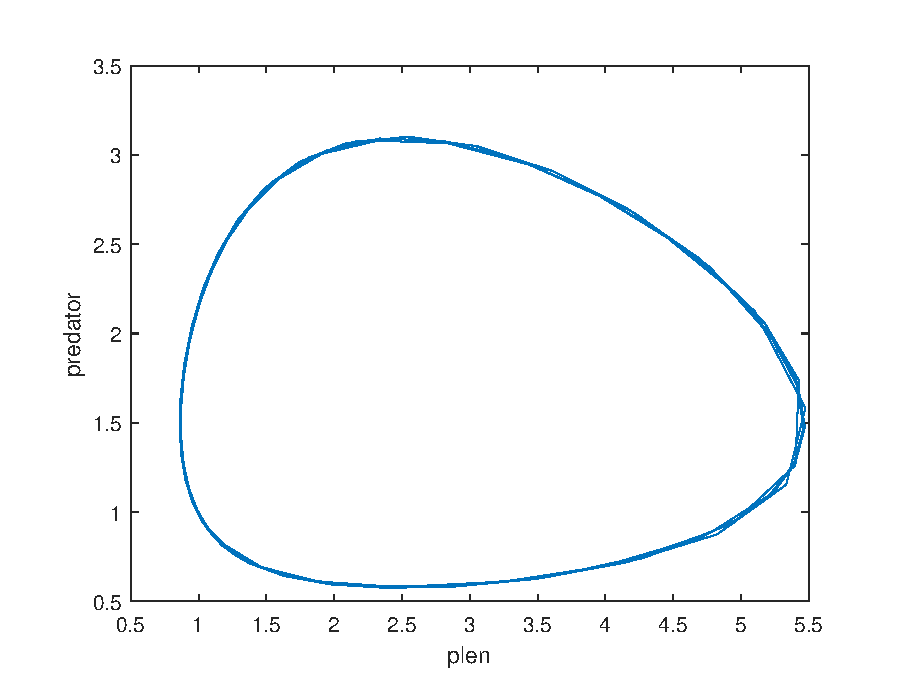
\includegraphics[width=1\textwidth]{images/lotka_voltera_phase} % first figure itself
        \caption{Fazni dijagram standardnog modela}
    \end{minipage}\hfill
    \begin{minipage}{0.45\textwidth}
        \centering
        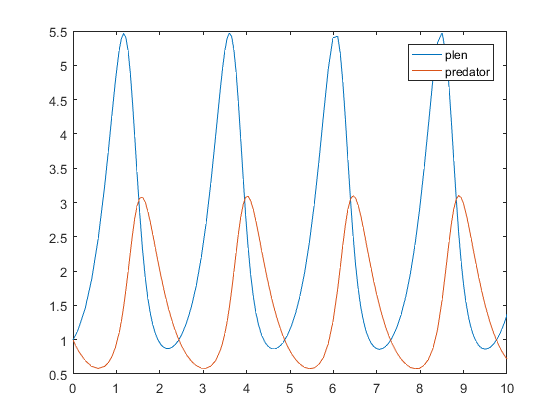
\includegraphics[width=1\textwidth]{images/lotka_voltera_time_plot} % second figure itself
        \caption{Grafik promene populacija kroz vreme za standardni model}
    \end{minipage}
\end{figure}

\section{Logistička modifikacija Lotka-Voltera modela}
\label{sec:log_mod}
Ukoliko je prirodni priraštaj negativan, populacija će eksponencijalno opadati ka nuli,
tj. težiće izumiranju. Ako je prirodni priraštaj pozitivan, populacija će da raste.
Može se videti da je ovaj model realističan sve dok je prirodni priraštaj konstantan.\\
Znamo da na realnom, konačnom staništu populacija ne može neograničeno rasti zbog
ograničenih raspoloživih resursa. Dakle, stanište može da podrži odredjen maksimalan broj
jedinki neke vrste. Označimo taj maksimum sa U. Kada ovaj maksimalni broj živi duže vreme u
nepromenjenom broju jasno je da je priraštaj u toj situaciji jednak nuli. Iskoristivši pretpostavku
da priraštaj linearno zavisi od veličine populacija, belgijski matemaričar Verhulst je predložio model:
	\begin{center}
		$\frac{dN(t)}{dt}=rN (t) (1 - \frac{N (t)}{U})$
	\end{center}
Mi smo iskoristili ovu jednačinu tako što smo zamenili u jednačini za plen deo
formule za priraštaj plena logističkom formulom. Time smo uračunali zavisnost
priraštaja od odnosa veličine populacije i kapaciteta staništa.\\

\subsection{Primer u Matlabu}
\label{sub:log_mod_matlab}

Fazni dijagram za modifikaciju modela formiramo pomoću m fajla $ logistic\_equations.m $, kada
trava ne može da ishrani više od U zečeva, gde nam je U parametar u logističkom modelu:

\lstinputlisting{../logistic_equations.m}

\begin{figure}[H]
    \centering
    \begin{minipage}{0.45\textwidth}
        \centering
        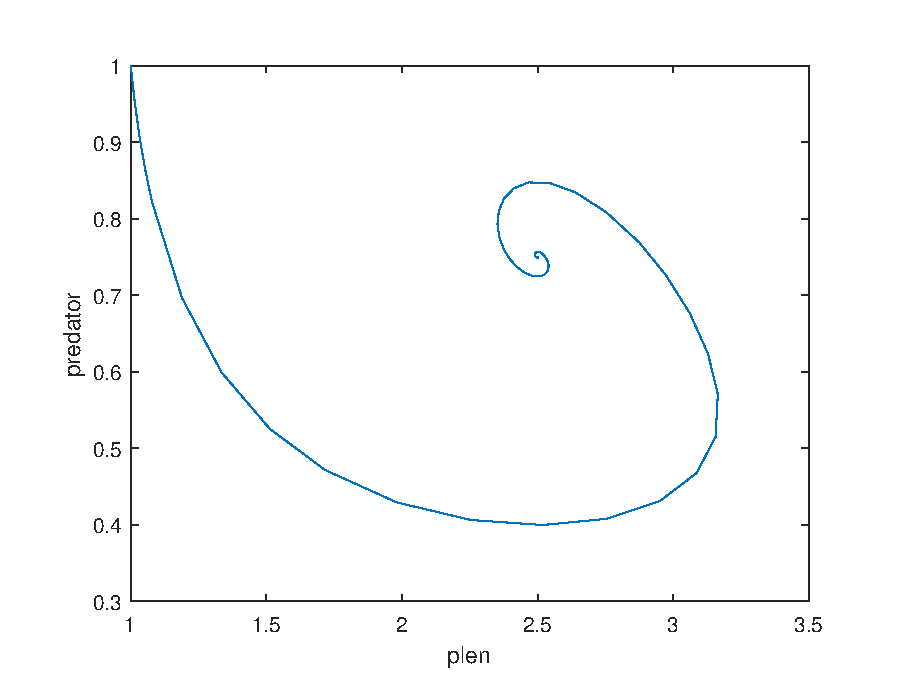
\includegraphics[width=1\textwidth]{images/lotka_voltera_logistic_phase} % first figure itself
        \caption{Fazni dijagram za U=5}
    \end{minipage}\hfill
    \begin{minipage}{0.45\textwidth}
        \centering
        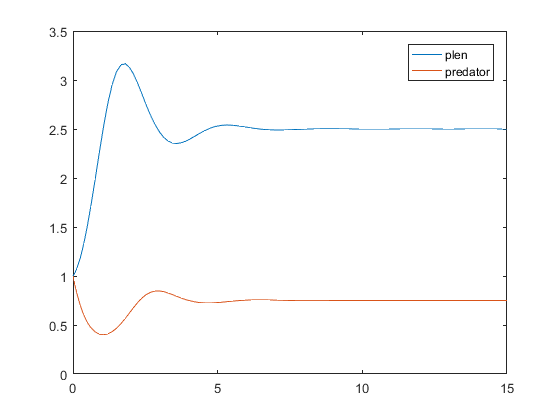
\includegraphics[width=1\textwidth]{images/lotka_voltera_logistic_time_plot} % second figure itself
        \caption{Promena populacija za U=5}
    \end{minipage}
\end{figure}


\subsection{Stanište sa vrlo ograničenim kapacitetom}
\label{sub:log_mod_ogr}

\begin{figure}[H]
    \centering
    \begin{minipage}{0.45\textwidth}
        \centering
        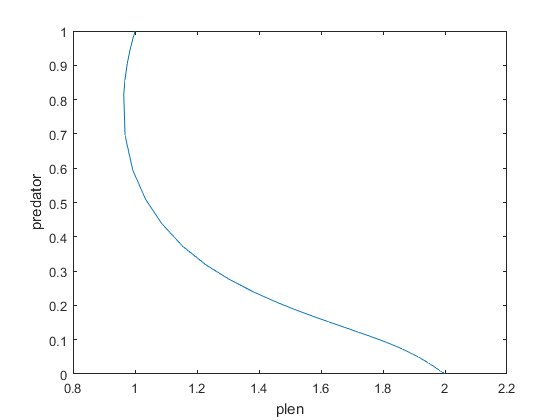
\includegraphics[width=1\textwidth]{images/lv_low_u_phase} % first figure itself
        \caption{Fazni dijagram za U=2}
    \end{minipage}\hfill
    \begin{minipage}{0.45\textwidth}
        \centering
        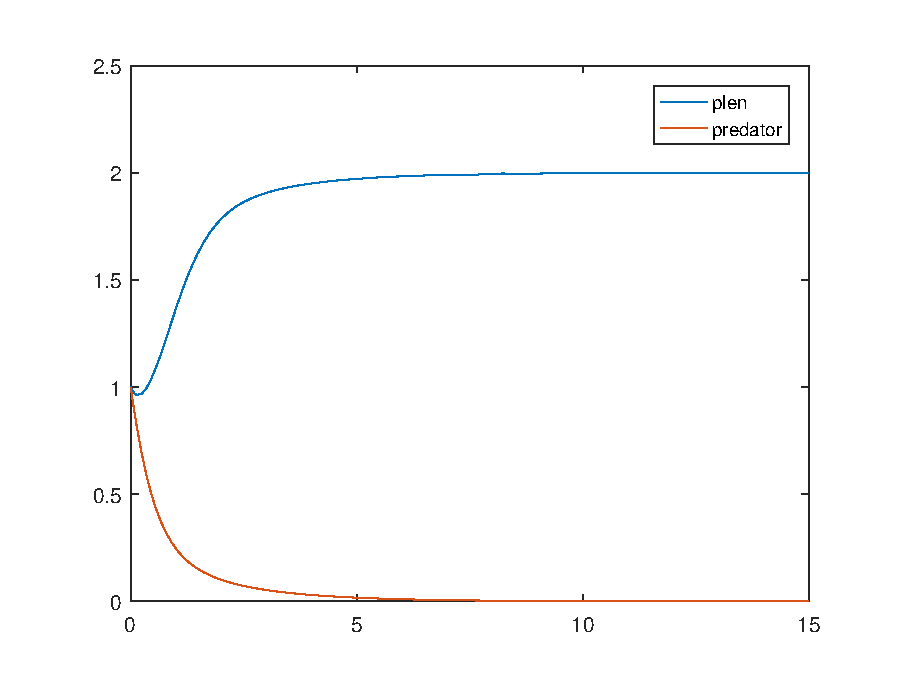
\includegraphics[width=1\textwidth]{images/lv_low_u_time} % second figure itself
        \caption{Promena populacija za U=2}
    \end{minipage}
\end{figure}

\section{Zaključak}
\label{sec:zakljucak}

Osnovni Lotka-Voltera model je dobar za modeliranje vrlo jednostavnih sistema,
ali kod kompleksnijih sistema, sa više interakcija i kompleksnijim parametrima ne uspeva
da realistišno predstavi situaciju. Sa druge strane, usled svoje elegancije i jednostavnosti,
izuzetno ga je lako modifikovati ili inkorporirati u druge modele, što ga čini relevantnim i danas.

\end{document}